\question{Câu 8}

Cho một tín hiệu cần xử lý dưới dạng dòng điện, có tầm thay đổi từ 1mA – 10mA. 

\answer{a}{Thiết kế mạch cho ngõ ra tầm 0\textsf{V} - 5\textsf{V}.}

\begin{minipage}{.5\linewidth}
	\begin{figure}[H]
		\centering
		
\includegraphics[width=\linewidth]{./my-chapters/my-images/Question8/debai.png}
	\end{figure}
\end{minipage}
\begin{minipage}{.5\linewidth}
	Thiết lập phương trình quan hệ giữa ngõ vào và ngõ ra:
	\[V_{out} = \dfrac{5000}{9}I_{in} - \dfrac{5}{9}\]
\end{minipage}

Ở đây dựa vào thiết kế của câu 7 ở trên ta có mạch như sau:

\begin{figure}[H]
	\centering
	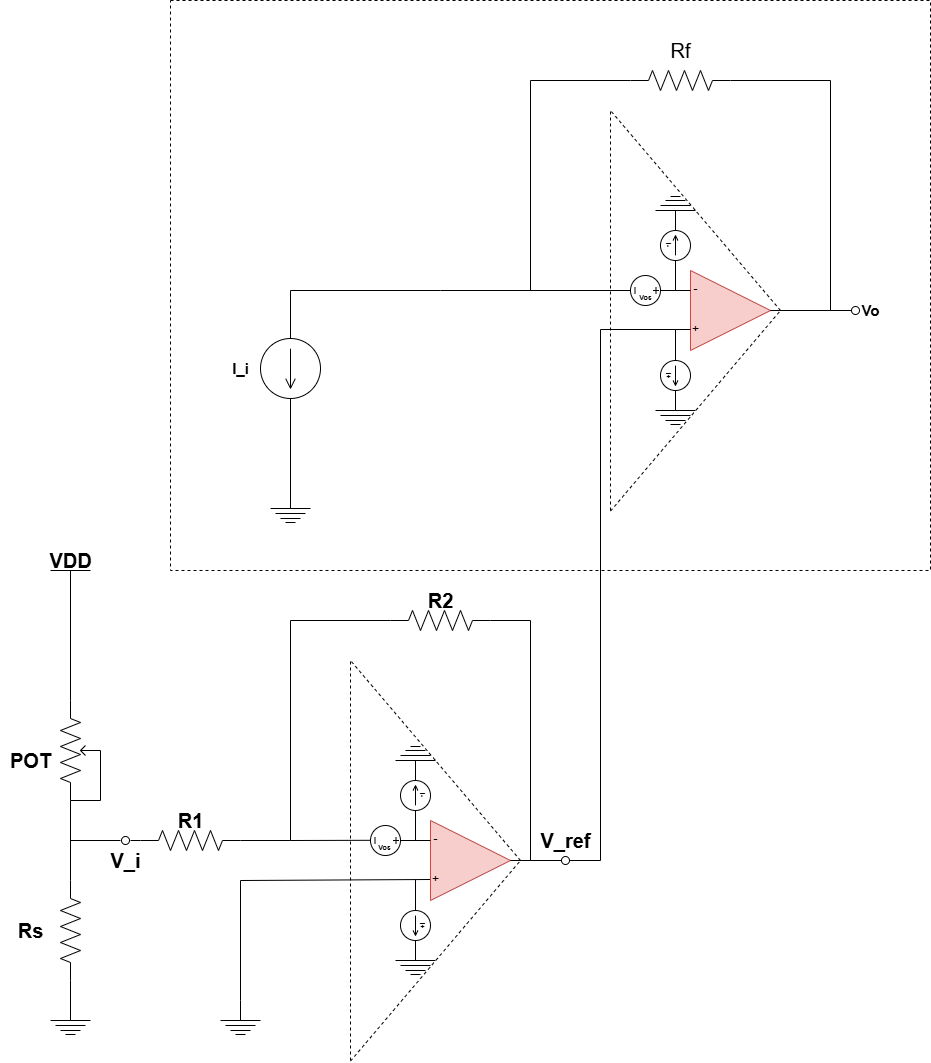
\includegraphics[width=.8\linewidth]{./my-chapters/my-diagrams/Question8/mach_tong.png}
	\caption{Transimpedance Amplifier với $V_{ref} \neq 0$.}
\end{figure}

$\Rightarrow \text{Chọn } R_{F} = \dfrac{5000}{9} \approx 560\,\Omega$

Tuy nhiên với ngõ vào $I_{in} = 1\,\textsf{mA}$ thì ở ngõ ra theo công thức của câu 7 sẽ là: $V_{out} = R_{F}I_{in} - V_{os} + I_{-}R_{F} = 560\times 1\,\textsf{mA} - 85\,\mu\textsf{V} + 560\times 3.1\,\textsf{nA} \approx 0.5599 \,\textsf{V}$. Vậy nên cần phải trừ đi một khoảng là $0.5599\,\textsf{V}$ tức là cộng thêm một lượng $V_{ref} \approx -0.5599\,\textsf{V}$.

$\Rightarrow$ \finalresult{V_{out} = R_{F}I_{in} - V_{os} + I_{-}R_{F} + V_{ref}}.

\subsubsection*{\textbf{Thực hiện mạch ở ngõ ra $\mathbf{V_{ref}}$}}

\begin{figure}[H]
	\centering
	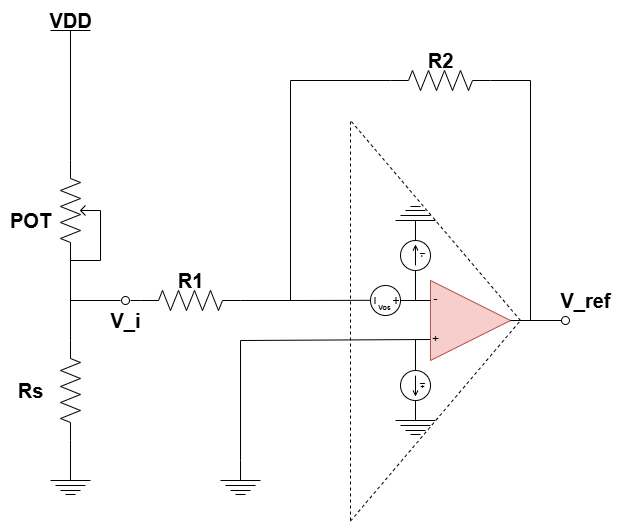
\includegraphics[width=.8\linewidth]{./my-chapters/my-diagrams/Question8/vref_schematric.png}
	\caption{Mạch thực điều khiển điện áp $V_{ref}$.}
\end{figure}

Ta xét ở tầng khuếch đại như sau:
\[ V_{ref} = -\dfrac{R_{2}}{R_{1}} V_{i}\]
Cho $V_{i} = 1\,\textsf{V}$ và $V_{ref} \approx -0.5599\,\textsf{V}$ thì $\dfrac{R_{2}}{R_{1}} = \dfrac{0.5599}{1} = 0.5599\,\textsf{V/V}$
\[\text{Chọn }R_{2} = 1\,\textsf{k}\Omega \Rightarrow R_{1} \approx 1.8\,\textsf{k}\Omega \]

Tiến hành mô phỏng Multisim để chọn ra được $V_{i} = 1\,\textsf{V}$

\begin{figure}[H]
	\centering
	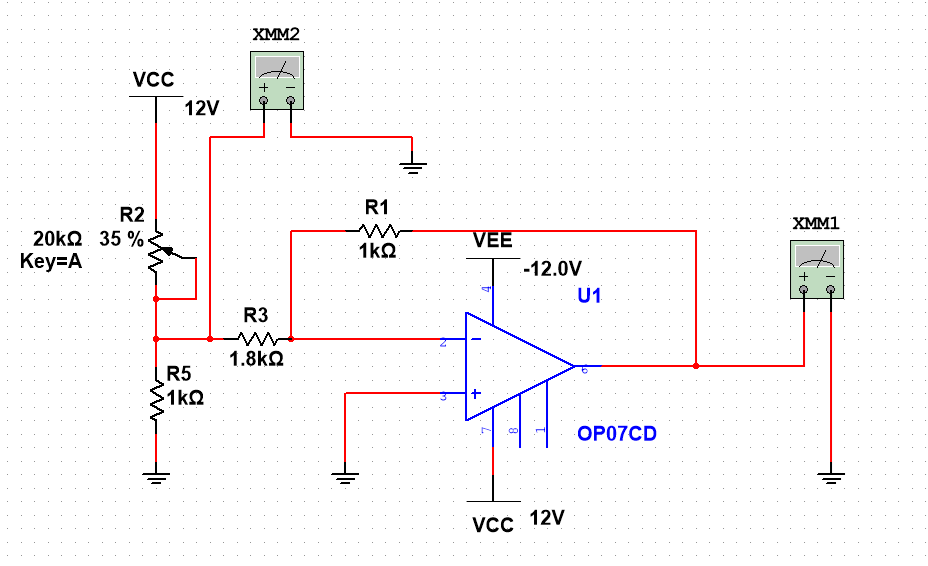
\includegraphics[width=.8\linewidth]{./my-chapters/my-images/Question8/a_find_V_i_Vref.png}
	\caption{Tìm giá trị $V_{i}$ giúp $V_{ref} \approx -0.5599\,\textsf{V}$.}
\end{figure}

Ta có kết quả như sau:

\begin{figure}[H]
	\centering
	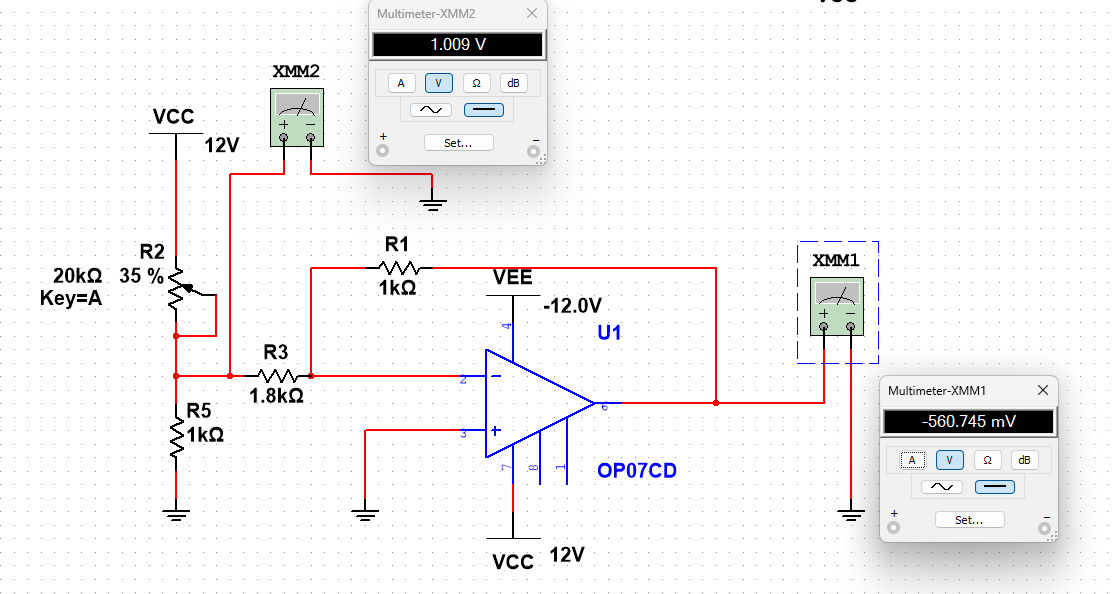
\includegraphics[width=.8\linewidth]{./my-chapters/my-images/Question8/a_result_V_i_Vref.png}
\end{figure}

Vậy với mạch trên cho ra $V_{ref} = -560.745\,\textsf{mV}$ nằm trong vùng chấp nhận được.

\answer{b}{Lựa chọn OPAMP và các linh kiện cần thiết để mạch hoạt động. Lưu ý: xử lý các thông số không lý tưởng của OPAMP. (Tham khảo datasheet)}

\begin{figure}[H]
	\centering
	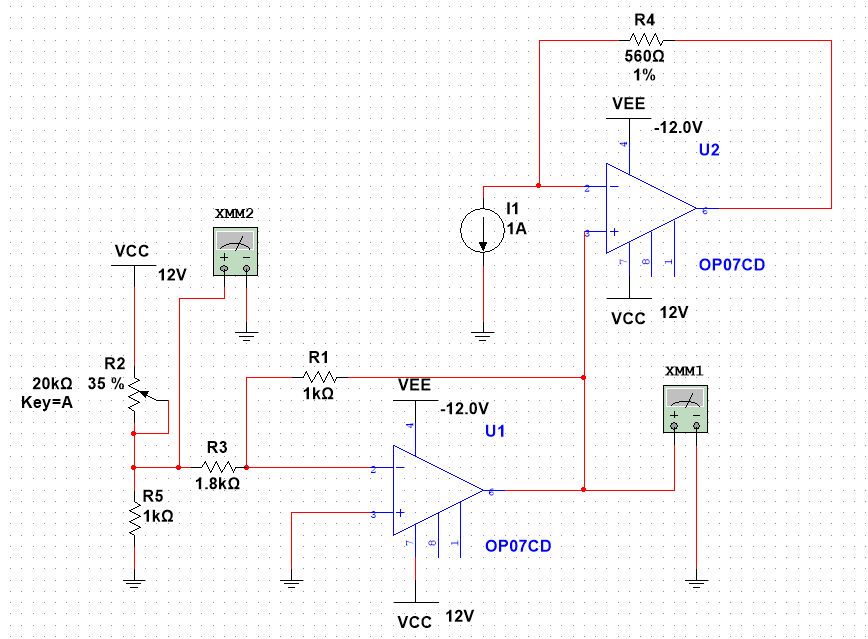
\includegraphics[width=0.7\linewidth]{my-chapters/my-images/Question8/b_mach_thiet_ke.png}
	\caption{Sơ đồ mạch của mạch Transimpedance Amplifier kèm $V_{ref}$.}
\end{figure}

Tiến hành DC sweep để đo điện áp ngõ ra khi điện áp ngõ vào thay đổi từ $1\,\textsf{mA} \rightarrow 10\,\textsf{mA}$,

\begin{figure}[H]
	\centering
	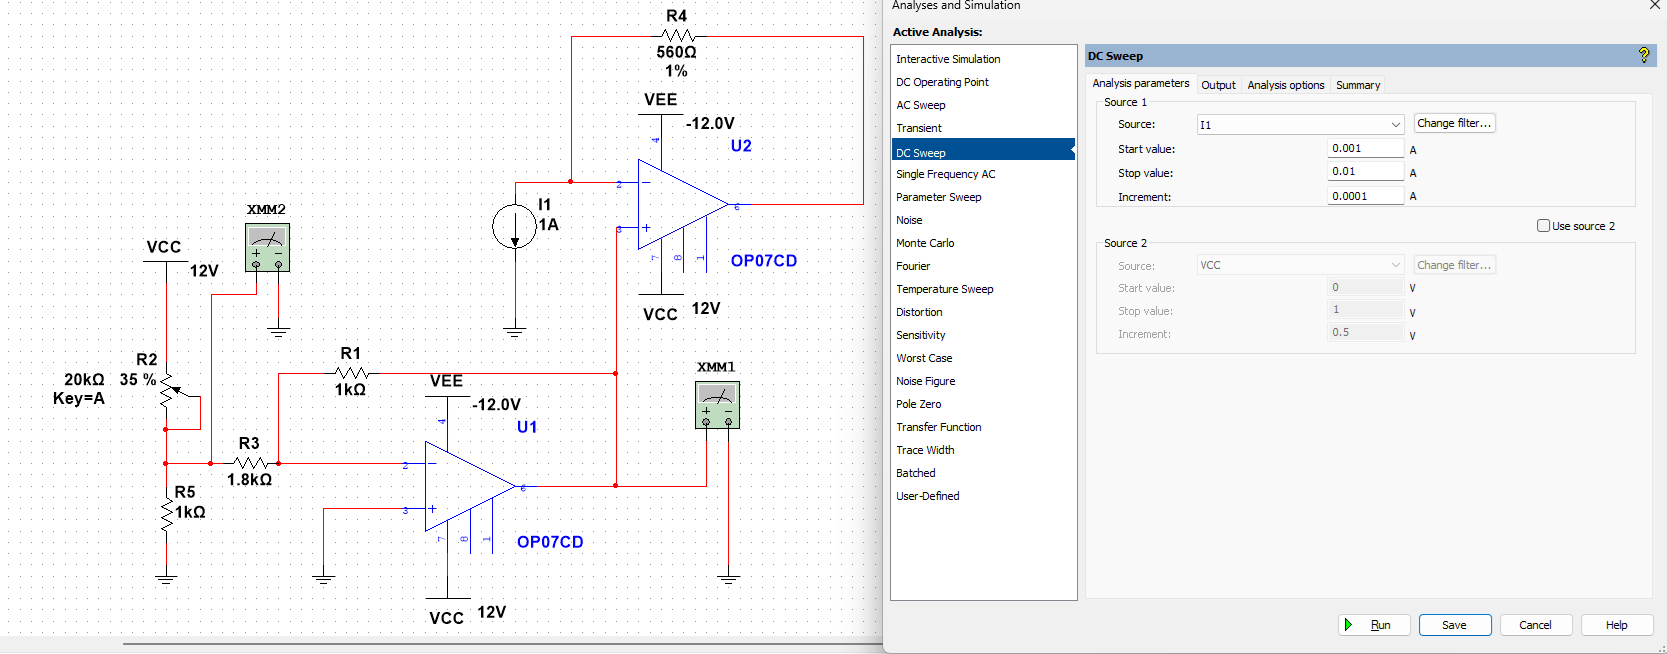
\includegraphics[width=0.7\linewidth]{my-chapters/my-images/Question8/b_dc_sweep.png}
	\caption{Tiến hành chạy DC swepp.}
\end{figure}

Kết quả,

\begin{figure}[H]
	\centering
	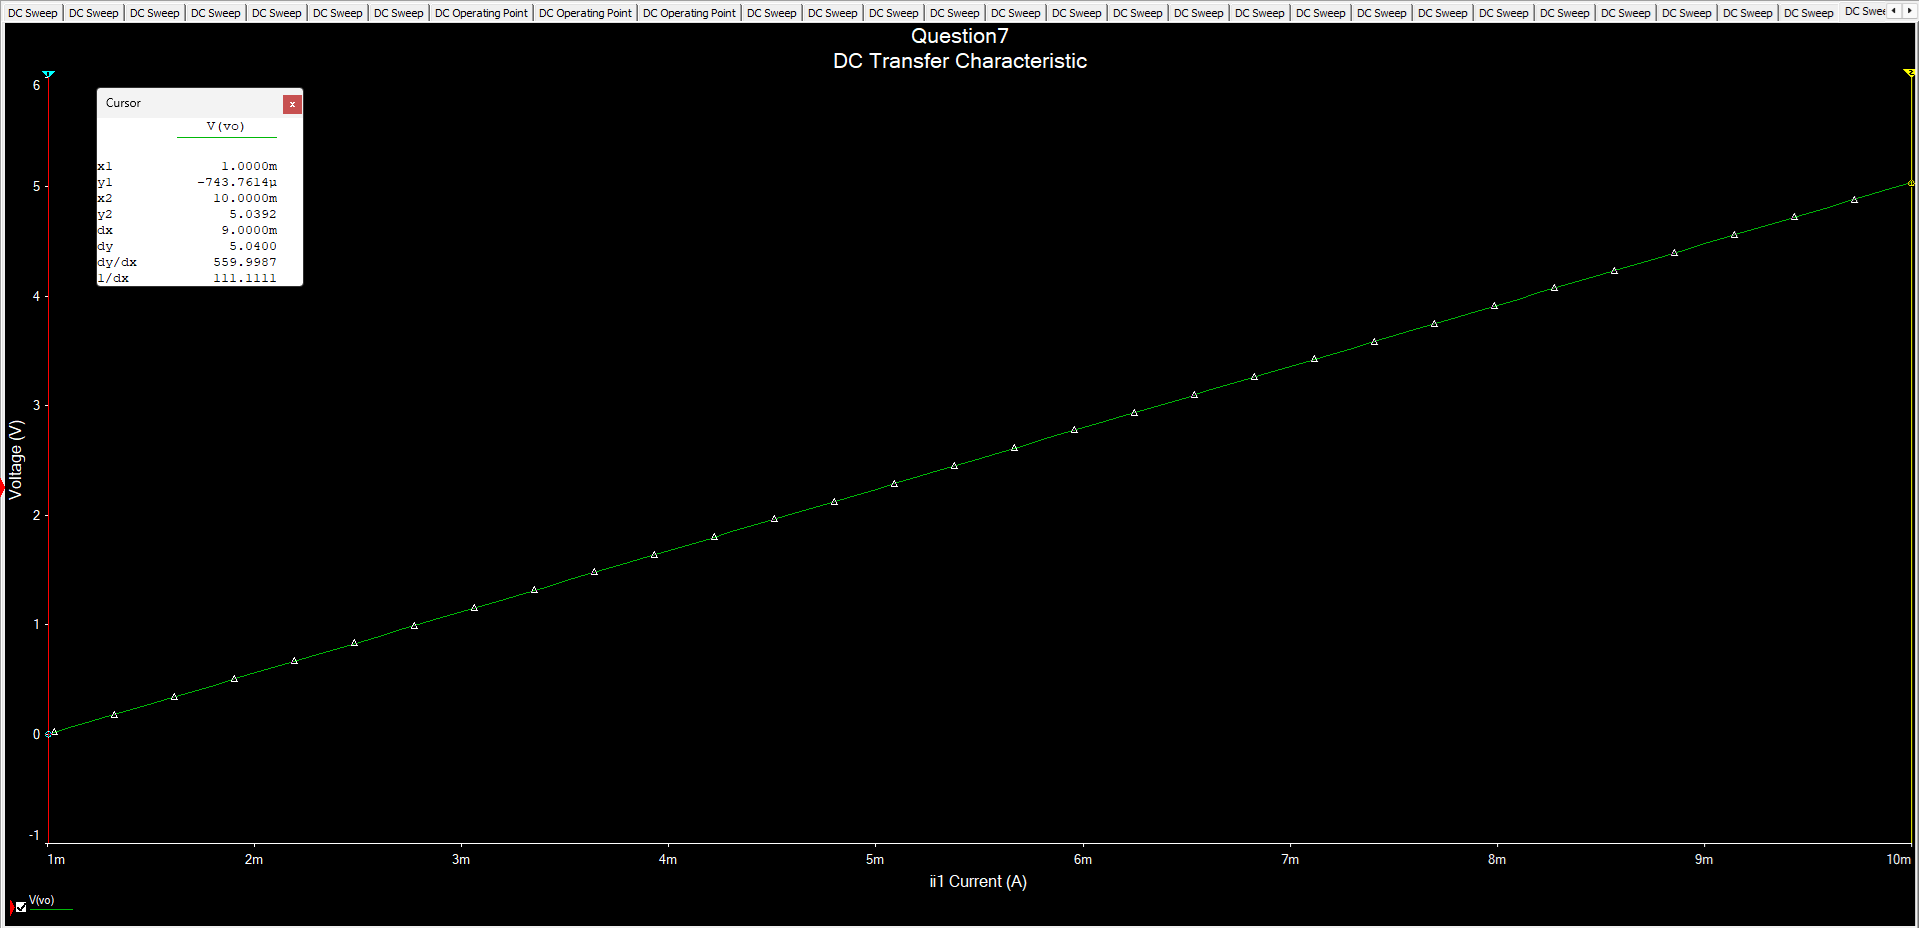
\includegraphics[width=\linewidth]{my-chapters/my-images/Question8/b_ketqua_dc_sweep.png}
	\caption{Kết quả của ngõ ra sau khi chạy DC sweep.}
\end{figure}

Kiểm tra sai số,

\begin{minipage}{.5\linewidth}
	\begin{figure}[H]
		\centering
		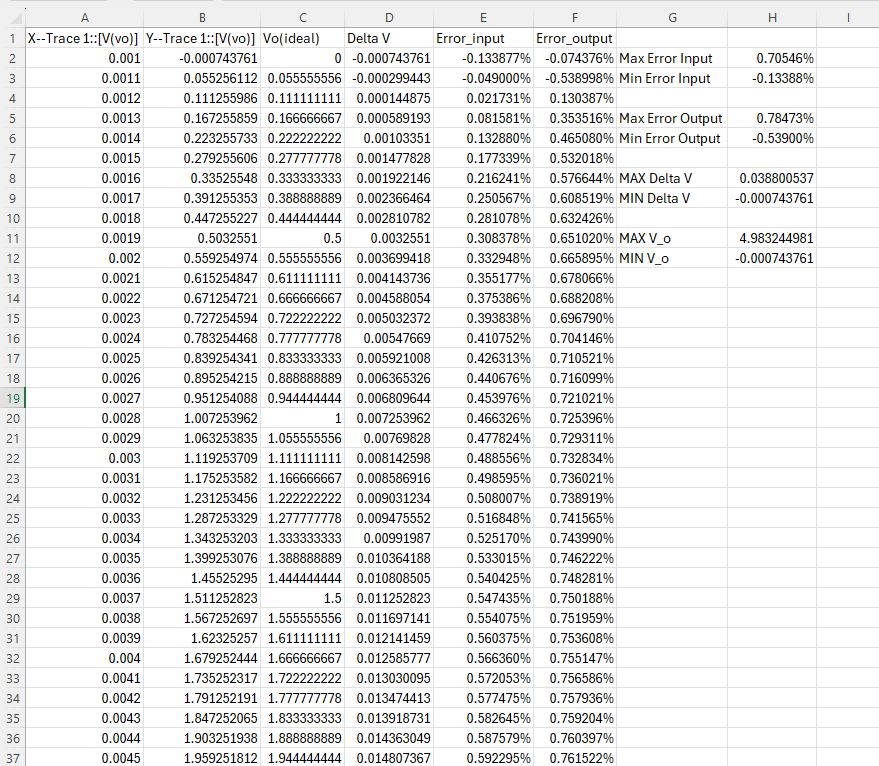
\includegraphics[width=\linewidth]{./my-chapters/my-images/Question8/b_saiso.png}
	\end{figure}
\end{minipage}
\begin{minipage}{.5\linewidth}
	\begin{itemize}[label=-]
		\item Giá trị $V_{ideal}$ được tính bằng cách lấy $I_{in}\times \dfrac{5000}{9} - \dfrac{5}{9}$
		\item Giá trị $\Delta V = V_{o} - V_{ideal}$
		\item Giá trị \finalresult{\Delta V _{max} =38.801\,\textsf{mV}} và \finalresult{\Delta V _{min} = -0.74\,\textsf{mV}}
		\item Sai số ở ngõ ra rơi vào tầm \finalresult{\Delta V_{o_{max}} = 0.78473\%} và \finalresult{\Delta V_{o_{min}} = -0.53900\%}
	\end{itemize}
\end{minipage}